%15.03.2024
\section{Lecture 6}

\begin{problem}[GHD - Gap Hamming Distance] \label{problem:GHD}
	Alice has $x \in \{0, 1\}^n$, Bob has $y \in \{0, 1\}^n$.
	Set $\alpha$ is some constant.
	
	Let's say that $\Delta(x, y)$ is a Hamming distance between those strings(count of positions in which $x$ and $y$ differ).
	
	Protocol should output 0 if $\Delta(x, y) < \frac n 2 - \alpha \sqrt n$ with $\Pr \geq 1 - \eps$.
	
	And protocol should output 1 if $\Delta(x, y) > \frac n 2 + \alpha \sqrt n$ with $\Pr \geq 1 - \eps$.
\end{problem}

\begin{remrk}
	Intuition is that $\frac n 2$ is average distance between two random strings.
	
	And $\sqrt n$ is standard deviation of distance between two random strings.
\end{remrk}

\begin{thm}
	$R_\eps(\text{GHD}) = \Omega(n)$.
\end{thm}

\begin{proof}
	The idea would be a reduction from INX \ref{problem:INX} to GHD \ref{problem:GHD}.
	
	Given INX instance $(x, i)$ we would construct GHD instance $(u, v)$ such that most probably their answers the same.
	
	Let's $r_1, \ldots, r_k \in \R^n$ be some random vectors uniformly distributed with property $| r_j|  = 1$.
	
	And define function $\text{sign}(x)$ equals to 1 when $x > 0$ and 0 otherwise.
	
	Define vectors $w$ and $e$:
	\begin{align*}
		w_j &= (-1)^{1 + x_j} = \begin{cases}
			1 &\iff x_j = 1 \\
			-1 &\iff \text{otherwise}
		\end{cases} \\
		e_j &= \begin{cases}
			0 &\iff i \neq j \\
			1 &\iff \text{otherwise}
		\end{cases}
	\end{align*}
	
	Now put
	\begin{align*}
		u_j &= \text{sign}(w \cdot r_j) \\
		v_j &= \text{sign}(e \cdot r_j)
	\end{align*}
	
	So $v_j$ is a sign of $i$th coordinate of $r_j$.
	The idea is that if $v_j$ equal to 1, then $u_j$ has more probability to be 1 than 0. 
	
	We want to calulate $\Pr[u_j = 1 \mid v_j = 1, x_i = 1]$.
	
	Let's note angle between $w$ and $e$, call that angle $\gamma$.
	\begin{align*}
		\cos \gamma = \frac{w \cdot e}{\|e\| \cdot \|w\|} =\frac {w \cdot e} {\sqrt n} = \frac 1 {\sqrt n}
	\end{align*}
	Last equality correct in under our conditions.
	
	Known fact that $\cos(\frac \pi 2 - x) \approx x$ we get that $\arccos(x) \approx \frac \pi 2 - x$.
	Implies that $\gamma \approx \frac \pi 2 - \frac{1}{\sqrt n}$.

	
	\begin{figure}[H]
		\centering
		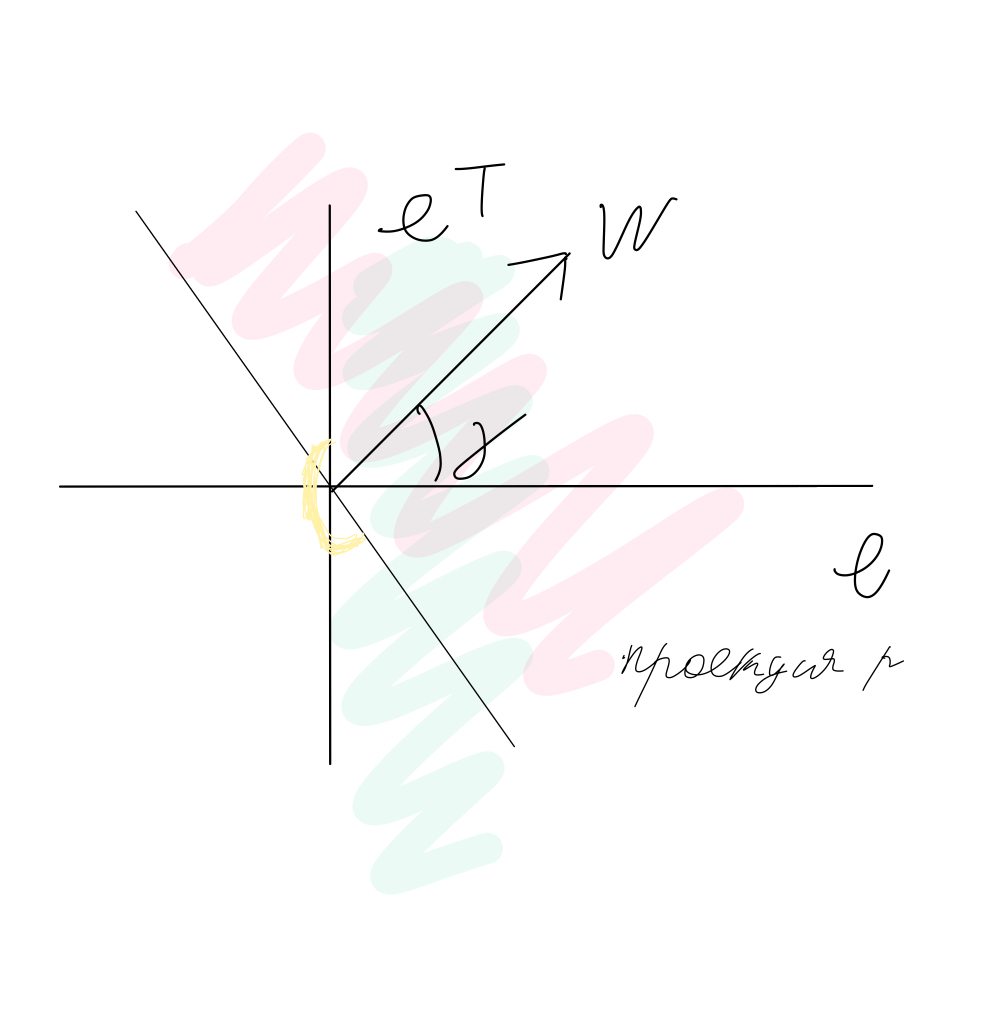
\includegraphics[width=0.4\linewidth]{figures/proof_ghd_projection.jpeg}
		\caption{Possible variants of projection vector $r$ onto $e$ plane.}
		\label{fig:proof_ghd_projection}
	\end{figure}
	
	
	If $u_j = 1 \implies \cos$ between $w$ and $r_j$ is positive, so area of $\gamma$ is $\gamma + 2(\frac \pi 2 - \gamma) = \pi - \gamma$(intersection of green and red on a picture). 
	So area is $\pi - \gamma  \approx \frac \pi 2 + \frac{1}{\sqrt n}$.

	Implies that $\Pr[u_j = 1 \mid v_j = 1, x_i = 1] \approx \frac{\frac \pi 2 + \frac{1}{\sqrt n}}{2 \pi}$.
	
	Implies that $\Pr[u_j = 1 \mid v_j = 1] = \frac{\pi + \Theta(\frac{1}{\sqrt n})}{2 \pi} = \frac 1 2 + \Theta(\frac 1 {\sqrt n})$.
	
	Similarly, we can show $\Pr[u_j = 1 \mid v_j = 1] = \frac 1 2 - \Theta(\frac{1}{\sqrt n})$.
	
	Let's estimate value of $k$.
	
	Summing over all coordinates we get:
	\begin{align*}
		\Pr\left[\left|\Delta(u, v) - \frac k 2\right|\right] = \Theta\left(\frac k {\sqrt n}\right)
	\end{align*}
	
	Implies that we need $k = \Theta(n)$.
	
	We will omit proof that not only average value is good.
	But we need to prove that with constant probability this happens.
	
	Which finishes our proof.

\end{proof}

Now we will try to get some lower bounds on Streaming Algorithms.

\begin{thm}[Lower bound for $F_0$]
	Exists $\beta, \delta$ such that $(\frac{\beta}{\sqrt n}, \delta)-F_0$ estimator requires $\Omega(n)$ space.
\end{thm}
\begin{proof}
	We would start with GHD \ref{problem:GHD} instance $x$ and $y$(of size $n$) and convert it to $F_0$ estimation with streams $\sigma_1$(from $x$) and $\sigma_2$(from $y$), such that if we can solve $F_0$ for $\sigma_1 \circ \sigma_2$ then we would get GHD answer.
	Sizes of $\sigma_1, \sigma_2$ would be linear.
	
	Put
	\begin{align*}
		\sigma_1[i] &= 2i + x_i \\
		\sigma_2[i] &= 2i + y_i
	\end{align*}
	
	Implies that $F_0(\sigma_1 \circ \sigma_2) = n + \Delta(x, y)$.
	
	We need to distinguish 
	\begin{align*}
		F_0 \begin{sqcases}
			> \frac{3n}{2} + \alpha n \\
			< \frac{3n}{2} - \alpha n
		\end{sqcases}
	\end{align*}
	
	Then exists $\beta, \delta$ such that $(\frac{\beta}{\sqrt n}, \delta)-F_0$ estimator requires $\Omega(n)$ space.
	
\end{proof}

\begin{remrk}
	Recall that we had an estimator for $(\eps, \delta)-F_0$ is solvable with space $O\left(\frac{1}{\eps^2} (\log^{O(1)}(n) + \log^{O(1)}(m))\right)$.
	And now we've proved tight lower bound!
\end{remrk}

\subsection{Compressed sensing}

Recall linear sketching.
Linear sketching is when we can say that our estimator just multiply some big matrix on vector of frequencies.

\begin{df}[CSSR - Compressed sensing Sparse recovery]

	Let's put $\text{res}_s(x) = \| x - x_s \|_{\mathcal L_1}$.
	
	Where
	\begin{align*}
		x_s[i] = \begin{cases}
			x[i] &\iff i \text{ in top $s$ coord} \\
			0 &\iff \text{otherwise}
		\end{cases}
	\end{align*}
	Top $s$ coord means that it's in the largest $s$ coordinates(if there is collision also sort lexicographical).
	
	For a fixed $s$ CSSR is an algorithm rec and matrix $A$ such that $\forall x$
	\begin{align*}
		\| \text{rec}(Ax) - x\|_{\mathcal L_1} \leq \alpha \cdot  \text{res}_s(x)
	\end{align*}
	
	So rec outputs some $x'$ that similar to $x$.
	Some kind of linear compression by multiplying on $A$ and after that recovering by rec.
\end{df}

\begin{thm}
	Assume some CSSR with $A \in M_{m \times n}$, then $m = \Omega\left(s \log \frac n s\right)$ for any $s = s(n)$.
\end{thm}
\begin{remrk}
	In our streaming algorithms $m$ is just space usage.
\end{remrk}
\begin{proof}
	We would use communication comlexity from Index problem(not everything is not randomized!).
	
	Alice has $x \in \{0, 1\}^n$ and Bob has $i \in [n]$.
	
	Let's choose such $|S|$ that $n = \log |S| \log n$ and $S \subseteq \{0, 1\}^t$ is a set of vectors such that
	\begin{align*}
		\forall v \neq u \in S \implies \Delta(u, v) \geq \frac t {10}
	\end{align*}, where $t = \Theta(\log |S|)$(such set exists for every $t$ due to probabilistic reasons).
	And also $\forall v \in S \implies v \neq \vec 0$.
	
	\begin{figure}[H]
	\centering
	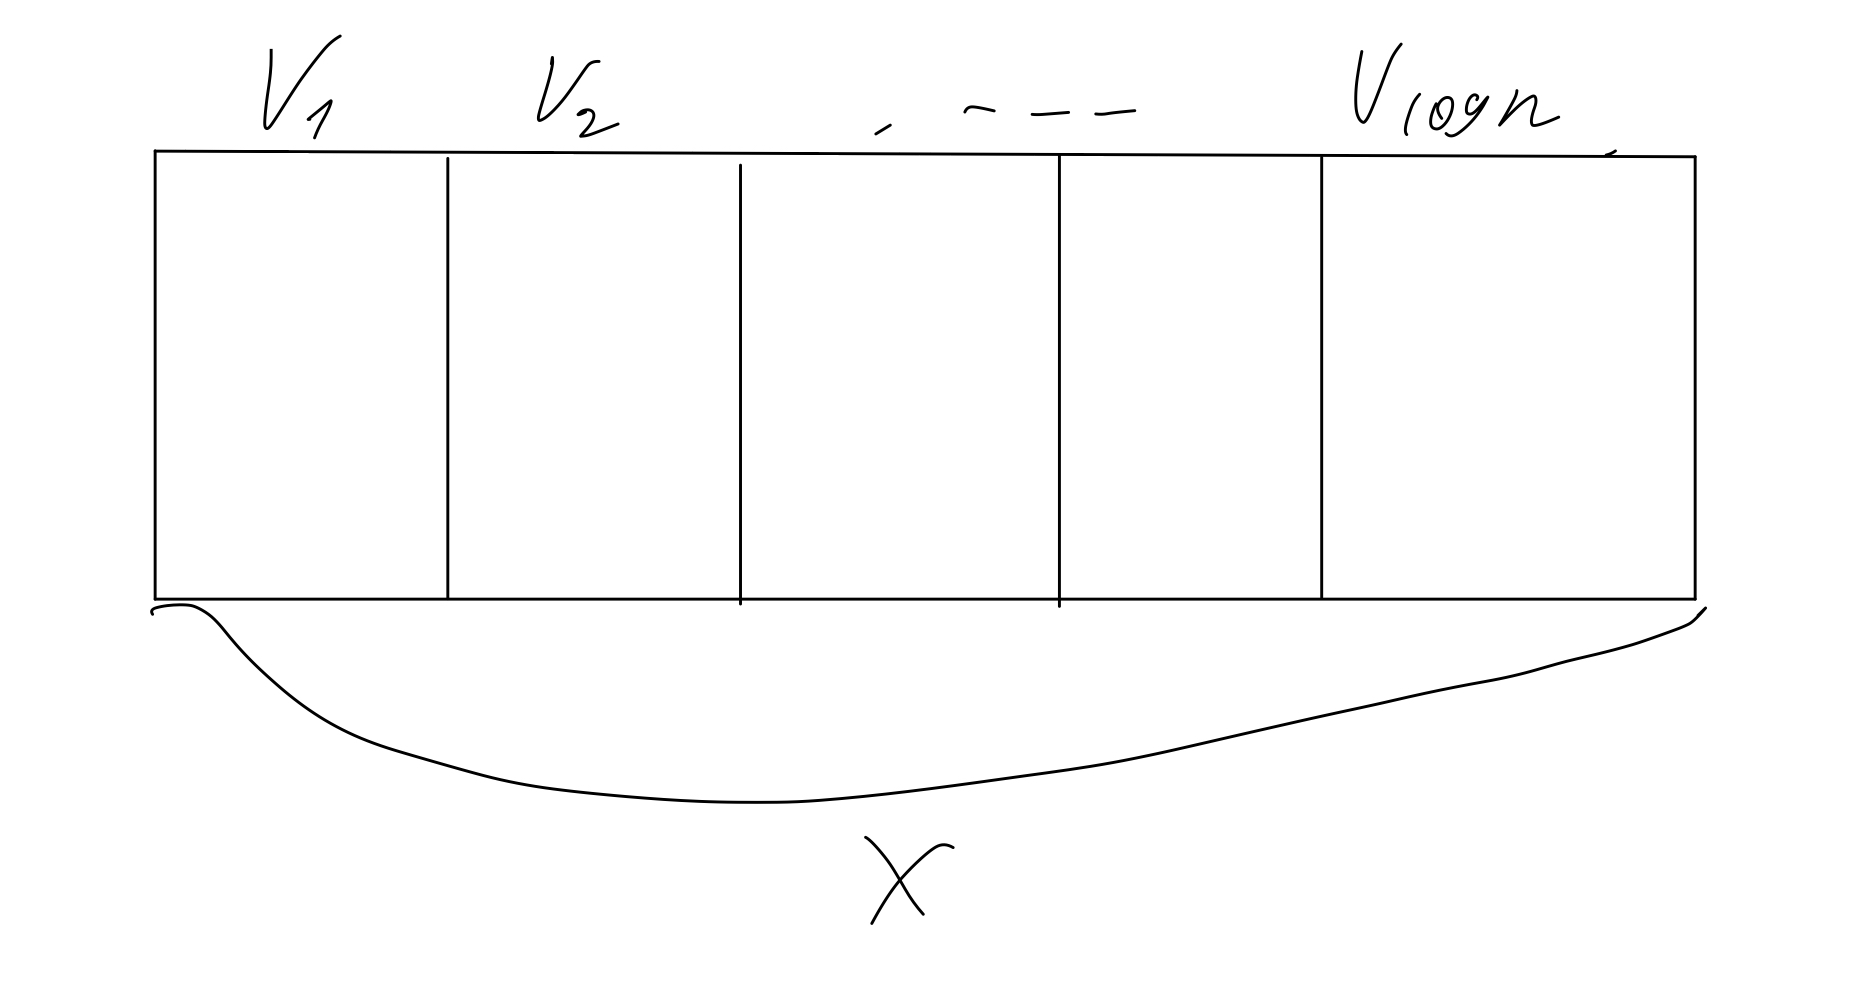
\includegraphics[width=0.4\linewidth]{figures/proof_cssr_blocks.jpeg}
	\caption{Partition of $x$ into blocks and after than transforming to $v_i$.}
	\label{fig:proof_cssr_blocks}
	\end{figure}
	
	So we take $i$th block of size $\log |S|$ from $x$, convert it to number, take element from $S$ by this index and it's our $v_i$.
	
	Alice would calculate
	\begin{align*}
		u = \sum_{i = 1}^{\log n} \alpha^i v_i
	\end{align*}, for some large constant $\alpha$.
	
	After that Alice sends $Au$ to Bob.
	Bob recovers $v_1, \ldots, v_{\log n}$ by rec algorithm.
	Bob can recover $v_{\log n}$ using formula:
	\begin{align*}
		v_{\log n} = u - \sum_{i = 1}^{\log n - 1} \alpha^i v_i
	\end{align*}
	If $v_{\log n}[i] = 1 \implies u_i \geq \alpha^{\log n}$ and if $v_{\log n}[i] = 0 \implies u_i \leq \sum_{i = 1}^{\log n - 1} \alpha^i < \alpha^{\log n}$.
	
	Implies that all positions where $v_{\log n}$ is 1 are also positions with 1 in $u$.
	
	Let $u' = \text{rec}(Au)$, we know that $\|u - u'\|_{\mathcal L_1} < c \cdot \text{res}_t(u)$.
	
	And let $v' = \alpha^{\log n} \cdot w$, where $w \in S$ such that $\| u' - v' \|_{\mathcal L_1}$ is $\min$.
	Implies that $v' = v_{\log n}$. Intuition of this is that distance between every two vectors in $S$ is huge. So if we take somebody else from $S$ then it would move as far away from $u'$.
	
	\begin{align*}
		\text{res}_t(u) \leq \sum_{i = 1}^{\log  n - 1} \alpha^i \|v_i\|_{\mathcal L_1}
	\end{align*}
	
	Because elements of $v_{\log n}$ would add a huge number to coordinates where $v_{\log n}$ is not zero and $t = |v_{\log n}|$.
	
		\begin{figure}[H]
		\centering
		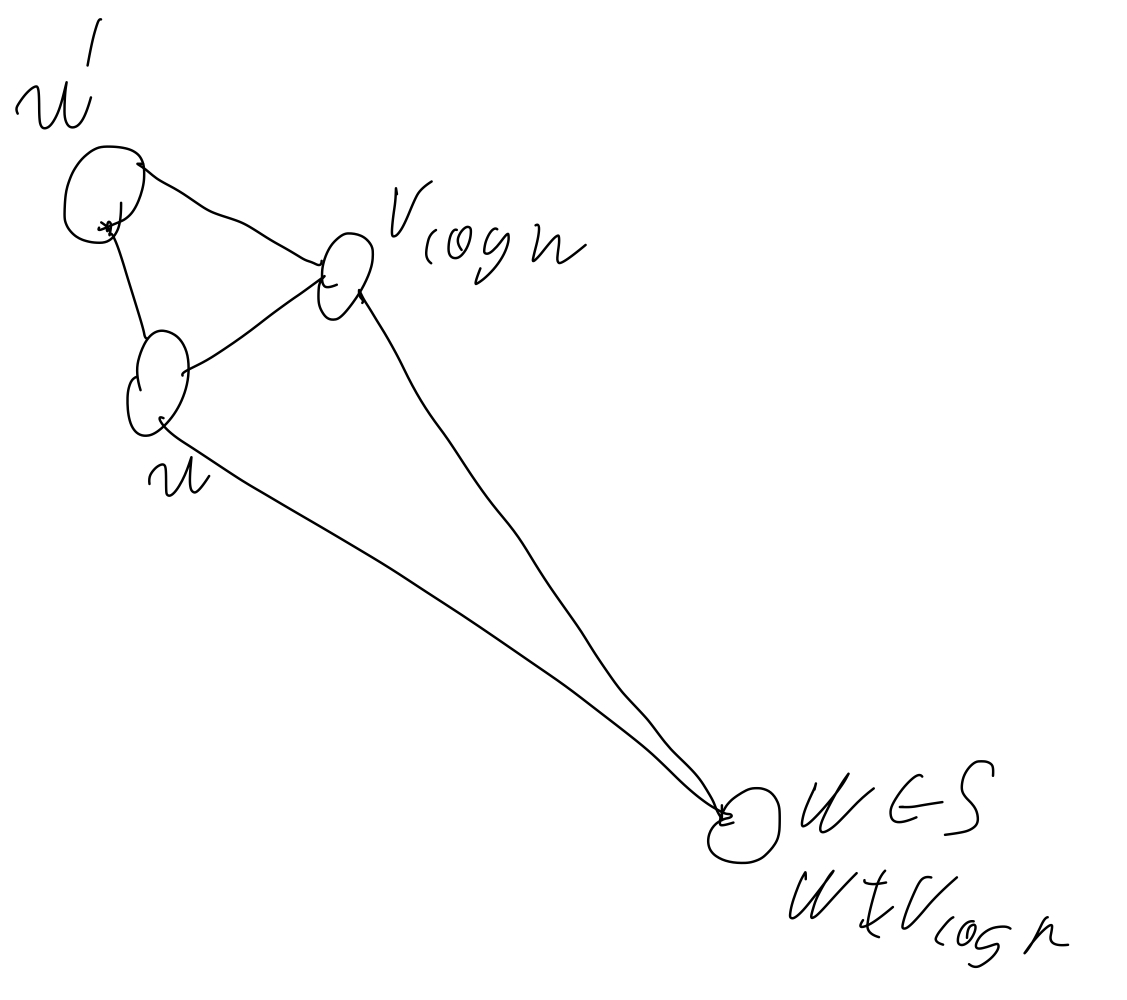
\includegraphics[width=0.4\linewidth]{figures/proof_cssr_distances.jpeg}
		\caption{$u'$ close to $u$ and $v_{\log n}$ close to $u$. While other $w \in S$ is far away from $v_{\log n}$, so $u'$ and $v_{\log n}$ is close.}
		\label{fig:proof_cssr_distances}
	\end{figure}
	
	After that we just run $\text{rec}(Au - A v_{\log n})$ and recover all $v_1, \ldots, v_{\log n}$.
	
	After that from $v_1, \ldots, v_{\log n}$ we can recover fully $x$ and output $x[i]$.
\end{proof}



